\documentclass[fleqn, a4paper, 11pt, oneside]{amsart}
\usepackage{exsheets, tasks}
\usepackage{amsmath, amssymb, amsthm} %standard AMS packages
\usepackage{marginnote} %marginnotes
\usepackage{gensymb} %miscellaneous symbols
\usepackage{commath} %differential symbols
\usepackage{xcolor} %colours
\usepackage{cancel} %cancelling terms
\usepackage{siunitx} %formatting units
\usepackage{tikz, pgfplots} %diagrams
\usetikzlibrary{calc, hobby, patterns, intersections}
\usepackage{graphicx} %inserting graphics
\usepackage{hyperref} %hyperlinks
\usepackage{datetime} %date and time
\usepackage{ulem} %underline for \emph{}
\usepackage{xfrac} %inline fractions
\usepackage{enumerate, enumitem} %numbered lists
\usepackage{float} %inserting floats
\usepackage{circuitikz} %circuit diagrams
\usepackage[noend]{algpseudocode}
\usepackage{algorithm}

\newcommand\numberthis{\addtocounter{equation}{1}\tag{\theequation}} %adds numbers to specific equations in non-numbered list of equations

\newcommand{\AxisRotator}[1][rotate=0]{
	\tikz [x=0.25cm,y=0.60cm,line width=.2ex,-stealth,#1] \draw (0,0) arc (-150:150:1 and 1);%
} %rotation symbols on axes

\theoremstyle{definition}
\newtheorem{example}{Example}
\newtheorem{definition}{Definition}

\theoremstyle{theorem}
\newtheorem{theorem}{Theorem}

\theoremstyle{remark}
\newtheorem{case}{Case}

\newcommand{\curl}{\mathrm{curl\,}}

\makeatletter
\@addtoreset{section}{part} %resets section numbers in new part
\makeatother

\makeatletter
\@addtoreset{case}{question} %resets section numbers in new part
\makeatother

\renewcommand{\thesubsection}{(\arabic{subsection})}
\renewcommand{\thesection}{(\arabic{section})}

\newcommand{\Not}{{\textsc{ not }}}
\renewcommand{\And}{{\textsc{ and }}}
\newcommand{\Or}{{\textsc{ or }}}
\newcommand{\Xor}{{\textsc{ xor }}}
\newcommand{\Nxor}{{\textsc{ nxor }}}
\newcommand{\Nand}{{\textsc{ nand }}}
\newcommand{\Nor}{{\textsc{ nor }}}

\newcommand{\AND}{\wedge}
\newcommand{\OR}{\vee}
\newcommand{\NOT}{\neg}
\newcommand{\XOR}{\oplus}

\newcommand{\logequiv}{\leftrightarrow}

\newcommand{\dual}{\mathrm{dual\,}}

%section headings on left
\makeatletter
\def\specialsection{\@startsection{section}{1}%
	\z@{\linespacing\@plus\linespacing}{.5\linespacing}%
	%  {\normalfont\centering}}% DELETED
	{\normalfont}}% NEW
\def\section{\@startsection{section}{1}%
	\z@{.7\linespacing\@plus\linespacing}{.5\linespacing}%
	%  {\normalfont\scshape\centering}}% DELETED
	{\normalfont\scshape}}% NEW
\makeatother

%forces newline after subsection
\makeatletter
\def\subsection{\@startsection{subsection}{3}%
	\z@{.5\linespacing\@plus.7\linespacing}{.1\linespacing}%
	{\normalfont\itshape}}
\makeatother

\newcommand{\strangesection}[1]{\renewcommand{\thesection}{#1}\section}
\newcommand{\strangesubsection}[1]{\renewcommand{\thesubsection}{#1}\subsection}

\settasks{counter-format = tsk[1].}

\SetupExSheets{solution/print = true}

%opening
\title{Digital Logic Systems : Assignment 5}
\author{
	Aakash Jog\\
	ID : 989323563\\
	\&\\
	Dustin Chalchinsky\\
	ID : 209741891\\
	\&\\
	Paul Mierau\\
	ID : 932384233
	}
\date{\formatdate{12}{5}{2015}}

\begin{document}
	
\maketitle
%\setlength{\mathindent}{0pt}

\begin{question}
	Design a zero-tester, defined as follows.\\
	\begin{tabular}{c c}
		Input         & $x[n - 1 : 0]$                  \\
		Output        & $y \in \{0,1\}$                 \\
		Functionality & $y = 1 \iff x[n - 1 : 0] = 0^n$ \\
	\end{tabular}
	\begin{enumerate}
		\item Suggest a design based on an $\Or$-tree.
		\item Suggest a design based on an $\And$-tree.
		\item What do you think about a design based on a tree of nor gates?
	\end{enumerate}
\end{question}

\begin{solution}
	\begin{enumerate}[leftmargin = *]
		\item
			The output must be $1$ if and only if all $n$ bits of the input are $0$.\\
			As $\Or$ is monotonic, at least one $\Not$ operator is necessary for implementation of the function.\\
			Therefore, as $0 \Or X \equiv X$, any tree can be made perfect by adding $0$s as inputs for completing the number of input bits to the smallest power of $2$ greater than or equal to $n$.
			\begin{figure}[H]
				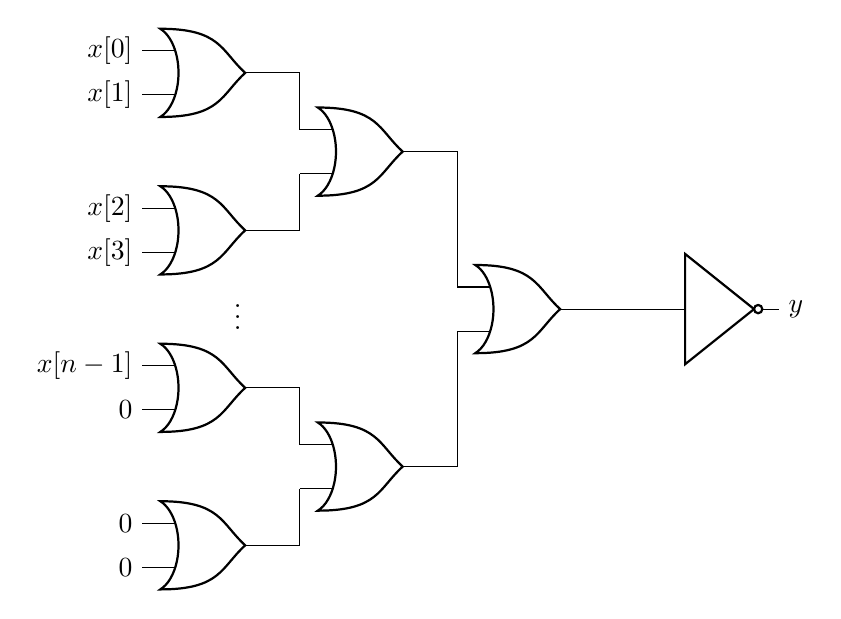
\begin{tikzpicture}
					\draw
						(0,6) node[or port] (or1) {}
						(0,4) node[or port] (or2) {}
						(0,2) node[or port] (or3) {}
						(0,0) node[or port] (or4) {}

						(2,5) node [or port] (or5) {}
						(2,1) node [or port] (or6) {}

						(4,3) node [or port] (or7) {}

						(6,3) node [not port] (not) {};

					\draw
						(or1.out) -| (or5.in 1)
						(or2.out) -| (or5.in 2);

					\draw
						(or3.out) -| (or6.in 1)
						(or4.out) -| (or6.in 2);

					\draw
						(or5.out) -| (or7.in 1)
						(or6.out) -| (or7.in 2);

					\draw
						(or7.out) -| (not.in);

					\node [left] at (0,3) {$\vdots$};

					\draw
						(or1.in 1) node[anchor=east] {$x[0]$}
						(or1.in 2) node[anchor=east] {$x[1]$}
						(or2.in 1) node[anchor=east] {$x[2]$}
						(or2.in 2) node[anchor=east] {$x[3]$}
						(or3.in 1) node[anchor=east] {$x[n - 1]$}
						(or3.in 2) node[anchor=east] {$0$}
						(or4.in 1) node[anchor=east] {$0$}
						(or4.in 2) node[anchor=east] {$0$}
						(not.out) node[anchor=west] {$y$};
				\end{tikzpicture}
			\end{figure}
		\item
			The output must be $1$ if and only if all $n$ bits of the input are $0$.\\
			As $\And$ is monotonic, at least one $\Not$ operator is necessary for implementation of the function.\\
			Therefore, as $1 \And X \equiv X$, any tree can be made perfect by adding $1$s as inputs for completing the number of input bits to the smallest power of $2$ greater than or equal to $n$.
			\begin{figure}[H]
				\begin{tikzpicture}
					\draw
						(0,14) node[not port] (not1) {}
						(0,12) node[not port] (not2) {}
						(0,10) node[not port] (not3) {}
						(0,8) node[not port] (not4) {}
						(0,6) node[not port] (not5) {};

					\draw
						(3,13) node[and port] (and1) {}
						(3,9) node[and port] (and2) {}
						(3,5) node[and port] (and3) {}
						(3,1) node[and port] (and4) {}

						(5,11) node[and port] (and5) {}
						(5,3) node[and port] (and6) {}

						(7,7) node [and port] (and7) {};

					\node [left] at (0,7) {$\vdots$};

					\draw
						(not1.in) node[anchor=east] {$x[0]$}
						(not2.in) node[anchor=east] {$x[1]$}
						(not3.in) node[anchor=east] {$x[2]$}
						(not4.in) node[anchor=east] {$x[3]$}
						(not5.in) node[anchor=east] {$x[n - 1]$}

						(and3.in 2) node[anchor=east] {$1$}
						(and4.in 1) node[anchor=east] {$1$}
						(and4.in 2) node[anchor=east] {$1$}

						(and7.out) node[anchor=west] {$y$};

					\draw
						(not1.out) -| (and1.in 1)
						(not2.out) -| (and1.in 2)
						(not3.out) -| (and2.in 1)
						(not4.out) -| (and2.in 2)
						(not5.out) -| (and3.in 1);
						
					\draw
						(and1.out) -| (and5.in 1)
						(and2.out) -| (and5.in 2)
						(and3.out) -| (and6.in 1)
						(and4.out) -| (and6.in 2);

					\draw
						(and5.out) -| (and7.in 1)
						(and6.out) -| (and7.in 2);
				\end{tikzpicture}
			\end{figure}
		\item
			As $\Or \equiv \Not(\Nor)$, a tree using $\Nor$ gates can be constructed by replacing all $\Or$ gates in the above tree by a combination of $\Nor$ and $\Not$ gates.
			\begin{figure}[H]
				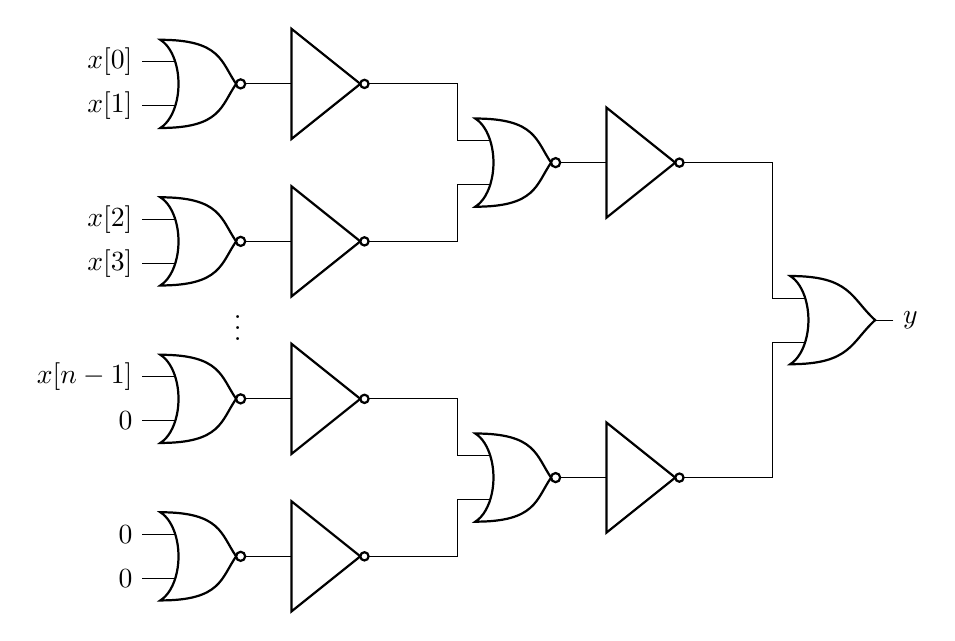
\begin{tikzpicture}
					\draw
						(0,6) node[nor port] (nor1) {}
						(1,6) node[not port] (not1) {}

						(0,4) node[nor port] (nor2) {}
						(1,4) node[not port] (not2) {}
						
						(0,2) node[nor port] (nor3) {}
						(1,2) node[not port] (not3) {}
						
						(0,0) node[nor port] (nor4) {}
						(1,0) node[not port] (not4) {}


						(4,5) node[nor port] (nor5) {}
						(5,5) node[not port] (not5) {}

						(4,1) node[nor port] (nor6) {}
						(5,1) node[not port] (not6) {}

						(8,3) node [or port] (or7) {};

					\draw
						(nor1.out) -| (not1.in)
						(nor2.out) -| (not2.in)
						(nor3.out) -| (not3.in)
						(nor4.out) -| (not4.in)
						(nor5.out) -| (not5.in)
						(nor6.out) -| (not6.in);

					\draw
						(not1.out) -| (nor5.in 1)
						(not2.out) -| (nor5.in 2)
						(not3.out) -| (nor6.in 1)
						(not4.out) -| (nor6.in 2);

					\draw
						(not5.out) -| (or7.in 1)
						(not6.out) -| (or7.in 2);

					\node [left] at (0,3) {$\vdots$};

					\draw
						(nor1.in 1) node[anchor=east] {$x[0]$}
						(nor1.in 2) node[anchor=east] {$x[1]$}
						(nor2.in 1) node[anchor=east] {$x[2]$}
						(nor2.in 2) node[anchor=east] {$x[3]$}
						(nor3.in 1) node[anchor=east] {$x[n - 1]$}
						(nor3.in 2) node[anchor=east] {$0$}
						(nor4.in 1) node[anchor=east] {$0$}
						(nor4.in 2) node[anchor=east] {$0$}
						(or7.out) node[anchor=west] {$y$};
				\end{tikzpicture}
			\end{figure}
	\end{enumerate}
\end{solution}

\begin{question}
	Prove that each of the following functions $f : \{0,1\}^n \to \{0,1\}$ is associative:
	\begin{enumerate}
		\item constant $0$
		\item constant $1$
		\item $x_1$
		\item $x_n$
		\item $\And_n$
		\item $\Or_n$
		\item $\Xor_n$
		\item $\Nxor_n$
	\end{enumerate}
\end{question}

\begin{solution}
	If $f ∶ \{0,1\}^2 \to \{0,1\}$ is an associative boolean function, then $f_n(x_1,x_2,\dots,x_n) = f\left( f_{n−k}(x_1,\dots,x_{n−k}),f_k(x_{n − k + 1},\dots,x_n) \right)$ for every $n \ge 2$ and $k \in [1,n − 1]$.\\
	Therefore, it is enough to show that the functions are associative for $2$ bits.\\
	\begin{enumerate}
		\item
			\begin{equation*}
				f(x_1,x_2,x_3) = 0
			\end{equation*}
			\begin{tabular}{|c|c|c||c|c|}
				\hline
				$x_1$ & $x_2$ & $x_3$ & $f((x_1,x_2),x_3)$ & $f(x_1,f(x_2,x_3))$ \\
				\hline
				0     & 0     & 0     & 0                  & 0                   \\
				0     & 0     & 1     & 0                  & 0                   \\
				0     & 1     & 0     & 0                  & 0                   \\
				0     & 1     & 1     & 0                  & 0                   \\
				1     & 0     & 0     & 0                  & 0                   \\
				1     & 0     & 1     & 0                  & 0                   \\
				1     & 1     & 0     & 0                  & 0                   \\
				1     & 1     & 1     & 0                  & 0                   \\
				\hline
	       		\end{tabular}\\
			Therefore, as the columns of $f((x_1,x_2),x_3)$ and $f(x_1,f(x_2,x_3))$ are identical, the function is associative.\\
		\item
			\begin{equation*}
				f(x_1,x_2,x_3) = 1
			\end{equation*}
			\begin{tabular}{|c|c|c||c|c|}
				\hline
				$x_1$ & $x_2$ & $x_3$ & $f((x_1,x_2),x_3)$ & $f(x_1,f(x_2,x_3))$ \\
				\hline
				0     & 0     & 0     & 1                  & 1                   \\
				0     & 0     & 1     & 1                  & 1                   \\
				0     & 1     & 0     & 1                  & 1                   \\
				0     & 1     & 1     & 1                  & 1                   \\
				1     & 0     & 0     & 1                  & 1                   \\
				1     & 0     & 1     & 1                  & 1                   \\
				1     & 1     & 0     & 1                  & 1                   \\
				1     & 1     & 1     & 1                  & 1                   \\
				\hline
			\end{tabular}\\
			Therefore, as the columns of $f((x_1,x_2),x_3)$ and $f(x_1,f(x_2,x_3))$ are identical, the function is associative.\\
		\item
			\begin{equation*}
				f(x_1,x_2,x_3) = x_1
			\end{equation*}
			\begin{tabular}{|c|c|c||c|c|}
				\hline
				$x_1$ & $x_2$ & $x_3$ & $f((x_1,x_2),x_3)$ & $f(x_1,f(x_2,x_3))$ \\
				\hline
				0     & 0     & 0     & 0                  & 0                   \\
				0     & 0     & 1     & 0                  & 0                   \\
				0     & 1     & 0     & 0                  & 0                   \\
				0     & 1     & 1     & 0                  & 0                   \\
				1     & 0     & 0     & 1                  & 0                   \\
				1     & 0     & 1     & 1                  & 0                   \\
				1     & 1     & 0     & 1                  & 0                   \\
				1     & 1     & 1     & 1                  & 0                   \\
				\hline
			\end{tabular}\\
			Therefore, as the columns of $f((x_1,x_2),x_3)$ and $f(x_1,f(x_2,x_3))$ are identical, the function is associative.\\
		\item
			\begin{equation*}
				f(x_1,x_2,x_3) = x_3
			\end{equation*}
			\begin{tabular}{|c|c|c||c|c|}
				\hline
				$x_1$  & $x_2$ & $x_3$ & $f((x_1,x_2),x_3)$ & $f(x_1,f(x_2,x_3))$ \\
				\hline
				0      & 0     & 0     & 0                  & 0                   \\
				0      & 0     & 1     & 1                  & 1                   \\
				0      & 1     & 0     & 0                  & 0                   \\
				0      & 1     & 1     & 1                  & 1                   \\
				1      & 0     & 0     & 0                  & 0                   \\
				1      & 0     & 1     & 1                  & 1                   \\
				1      & 1     & 0     & 0                  & 0                   \\
				1      & 1     & 1     & 1                  & 1                   \\
				\hline
			\end{tabular} \\
			Therefore, as the columns of $f((x_1,x_2),x_3)$ and $f(x_1,f(x_2,x_3))$ are identical, the function is associative.\\
		\item
			\begin{equation*}
				f(x_1,x_2,x_3) = x_1 \AND x_2 \AND x_3
			\end{equation*}
			\begin{tabular}{|c|c|c||c|c|}
				\hline
				$x_1$  & $x_2$ & $x_3$ & $f((x_1,x_2),x_3)$ & $f(x_1,f(x_2,x_3))$ \\
				\hline
				0      & 0     & 0     & 0                  & 0                   \\
				0      & 0     & 1     & 0                  & 0                   \\
				0      & 1     & 0     & 0                  & 0                   \\
				0      & 1     & 1     & 0                  & 0                   \\
				1      & 0     & 0     & 0                  & 0                   \\
				1      & 0     & 1     & 0                  & 0                   \\
				1      & 1     & 0     & 0                  & 0                   \\
				1      & 1     & 1     & 1                  & 1                   \\
				\hline
			\end{tabular} \\
			Therefore, as the columns of $f((x_1,x_2),x_3)$ and $f(x_1,f(x_2,x_3))$ are identical, the function is associative.\\
		\item
			\begin{equation*}
				f(x_1,x_2,x_3) = x_1 \OR x_2 \OR x_3
			\end{equation*}
			\begin{tabular}{|c|c|c||c|c|}
				\hline
				$x_1$  & $x_2$ & $x_3$ & $f((x_1,x_2),x_3)$ & $f(x_1,f(x_2,x_3))$ \\
				\hline
				0      & 0     & 0     & 0                  & 0                   \\
				0      & 0     & 1     & 1                  & 1                   \\
				0      & 1     & 0     & 1                  & 1                   \\
				0      & 1     & 1     & 1                  & 1                   \\
				1      & 0     & 0     & 1                  & 1                   \\
				1      & 0     & 1     & 1                  & 1                   \\
				1      & 1     & 0     & 1                  & 1                   \\
				1      & 1     & 1     & 1                  & 1                   \\
				\hline
			\end{tabular} \\
			Therefore, as the columns of $f((x_1,x_2),x_3)$ and $f(x_1,f(x_2,x_3))$ are identical, the function is associative.\\
		\item
			\begin{equation*}
				f(x_1,x_2,x_3) = x_1 \XOR x_2 \XOR x_3
			\end{equation*}
			\begin{tabular}{|c|c|c||c|c|}
				\hline
				$x_1$  & $x_2$ & $x_3$ & $f((x_1,x_2),x_3)$ & $f(x_1,f(x_2,x_3))$ \\
				\hline
				0      & 0     & 0     & 0                  & 0                   \\
				0      & 0     & 1     & 1                  & 1                   \\
				0      & 1     & 0     & 1                  & 1                   \\
				0      & 1     & 1     & 0                  & 0                   \\
				1      & 0     & 0     & 1                  & 1                   \\
				1      & 0     & 1     & 0                  & 0                   \\
				1      & 1     & 0     & 0                  & 0                   \\
				1      & 1     & 1     & 0                  & 0                   \\
				\hline
			\end{tabular} \\
			Therefore, as the columns of $f((x_1,x_2),x_3)$ and $f(x_1,f(x_2,x_3))$ are identical, the function is associative.\\
		\item
			\begin{equation*}
				f(x_1,x_2,x_3) = x_1 \Nxor x_2 \Nxor x_3
			\end{equation*}
			\begin{tabular}{|c|c|c||c|c|}
				\hline
				$x_1$  & $x_2$ & $x_3$ & $f((x_1,x_2),x_3)$ & $f(x_1,f(x_2,x_3))$ \\
				\hline
				0      & 0     & 0     & 1                  & 1                   \\
				0      & 0     & 1     & 0                  & 0                   \\
				0      & 1     & 0     & 0                  & 0                   \\
				0      & 1     & 1     & 1                  & 1                   \\
				1      & 0     & 0     & 0                  & 0                   \\
				1      & 0     & 1     & 1                  & 1                   \\
				1      & 1     & 0     & 1                  & 1                   \\
				1      & 1     & 1     & 1                  & 1                   \\
				\hline
			\end{tabular} \\
			Therefore, as the columns of $f((x_1,x_2),x_3)$ and $f(x_1,f(x_2,x_3))$ are identical, the function is associative.\\
	\end{enumerate}
\end{solution}

\begin{question}
	Prove that there is only one minimum depth binary tree with $n$ leaves if and only if $n$ is a power of $2$.
\end{question}

\begin{solution}
	If $n$ is a power of $2$, then the minimum depth tree is a perfect tree.
	Therefore, it is symmetrical for any arrangement of the leaves.\\
	Therefore, the tree is unique.\\
	~\\
	Conversely, let the minimum depth binary tree be unique.\\
	If possible, let $n$ not be a power of $2$.\\
	Therefore, the minimum depth tree is not perfect.\\
	Therefore, it is not symmetric with respect to the leaves.
	Hence, there can exist multiple trees with minimum depth.\\
	This contradicts the assumption the tree is unique.\\
	Therefore, $n$ must be a power of $2$.
\end{solution}

\end{document}
